\begin{frame}[label = nguyentu]{Cấu tạo nguyên tử}

Cấu tạo nguyên tử:

\begin{tikzpicture}
\node[draw](A) at (0,0){Atom};
\node[draw](B) at (15:4){Nucleus};
\node[draw](C) at (-15:5){electron};
\draw[->](A)|-(B);
\draw[->](A)-|(C);
\only<2->{\draw[->](A)edge[bend left](B);}
\only<2->{\draw[->](A)edge[bend right](C);}
\only<3->{\draw[->](B)edge[out=270, in=180](C);}
\end{tikzpicture}

\end{frame}